\subsection{Product Perspective}
% Introductory text describing system's integration with other products, considering shared phenomena.

% Text for Class Diagram
% Class diagram

% TODO: @Ozan If have time start this.

% For each core feature (which are they? all?):
%   - Scenario
%   - State Chart
%   - Explanation

% TODO: @Ozan go with these.
% Core features: Future book line number, now retrieve line number, Guest arrives to store, System stop (Shop's on fire), schedule system stop (don't forget to notify customer),
\subsubsection{Book Line Number}
\textbf{Scenario}
Ozan wants to visit the new hamburger place that has recently opened just around the corner of his house.
However, Ozan doesn't want to wait on a long line to purchase a burger and some fries.
The fast food joint has incorporated the CLup system in their customer service portfolio, making it possible to Ozan to reserve his ticket beforehand without visiting the location.
Ozan downloads the CLup app and books his line number from his house.
Using the app, he can plan his route and schedule to the location beforehand and place his order directly upon his arrival.

\textbf{State Chart}

\begin{figure}[H]
    \centering
    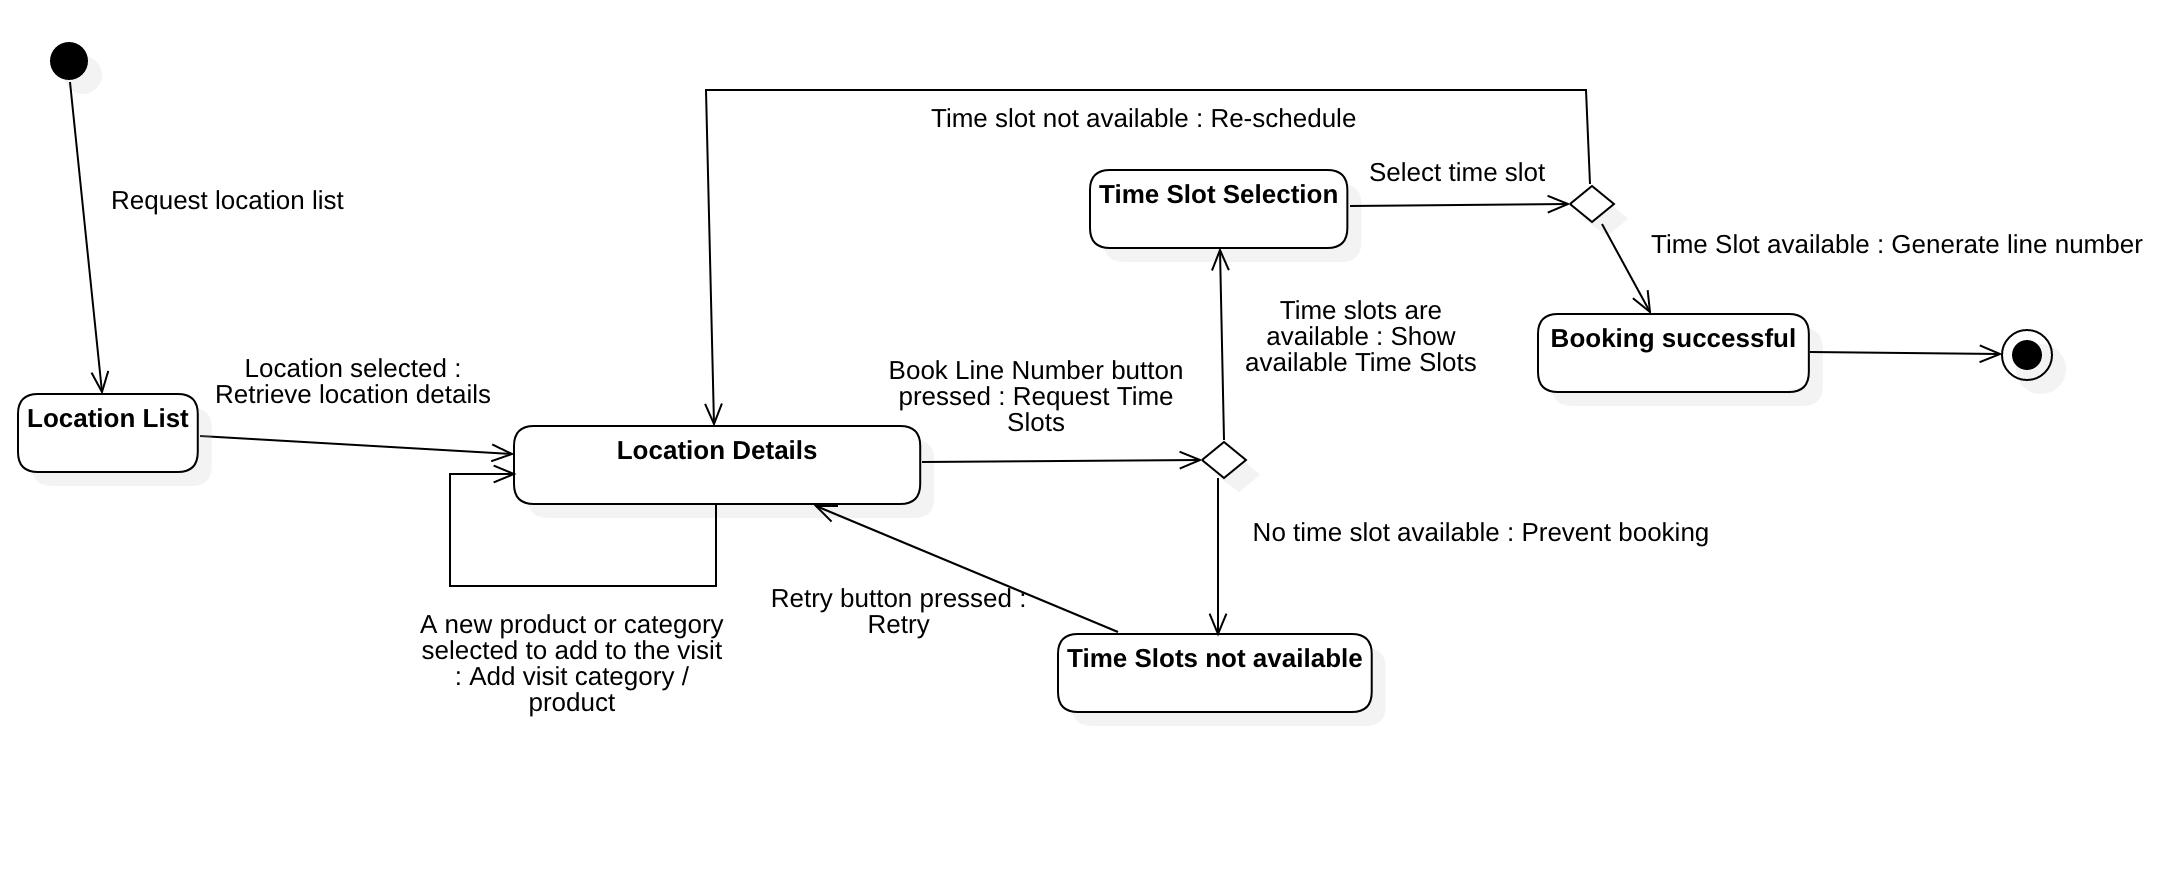
\includegraphics[height=0.4\textwidth]{Images/StateCharts/BookLineNumber.png}
    \caption{State Diagram for feature Book Line Number}
    \label{fig:SDBookLine}
\end{figure}

The \nameref{fig:SDBookLine} represents the execution flow of one of the core use cases, namely booking a line number for the future.
The customer books the line number by first listing what locations are available for them to book.
Then, when customer selects a location they view the details of the location, where they can add products or product categories to their target visit.
The customer can then view the time slots that the system will generate specifically filtered for their visit based on the provided data and availability of the location.
When the customer selects a specific time slot the system tries to book that specific location for the customer.
If the system successfully allocates the desired time slot, it displays the success message along the customer's ticket.
Else the user is notified of the failure and brought back to the scheduling screen for selection of another slot.


\subsubsection{Get Line Number}

\textbf{Scenario}

Roberto is living in Milan during the COVID lockdown and wants to visit a grocery store near his house.
He wants to obtain a line number for his visit through his phone to not waste time while waiting in the line for other customers to be done with their affairs.
He hears that the store he plans to visit has been on CLup, so he downloads the app and opens it.
Using the app, Roberto can now see when exactly he should take off to reach the shop without waiting in front of the store.

\textbf{State Chart}

\begin{figure}[H]
    \centering
    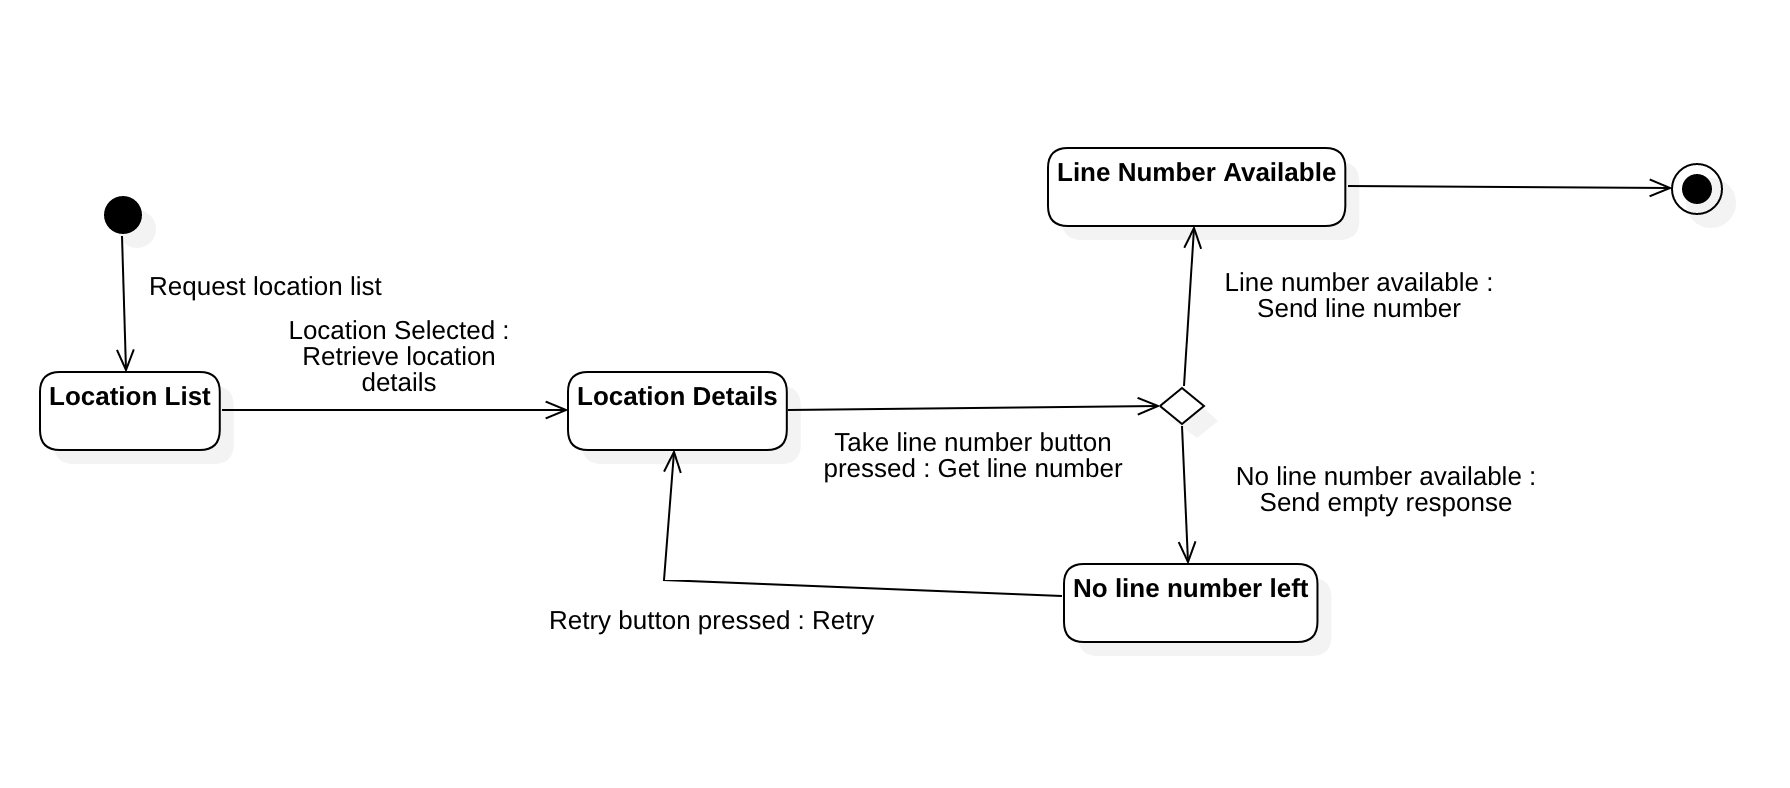
\includegraphics[height=0.4\textwidth]{Images/StateCharts/GenerateLineNumber.png}
    \caption{State Diagram for feature Get Line Number}
    \label{fig:SDGetLine}
\end{figure}

The \nameref{fig:SDGetLine} represents the execution flow of another core use case, booking a line number for a recent visit.
The customer generates a line number by going over the list of available locations, similar to the Book Line Number feature, however this time they press the "Take Line Number" button directly.
Then, the system tries to generate a line number for them, and if it is successful, the user retrieves the resulting line number.
If the system can not fulfill the user's request, it communicates the problem to the user and allows a retry.

\subsubsection{Print Line Number}

\textbf{Scenario}

Hrvoje, a Croatian recently arrived in Italy, is not aware of the popularity of CLup app, however wants to visit an electronics store to purchase a new phone, because his current phone has died out of battery failure.
Upon arrival, since he doesn't have a phone, he can not register to CLup system, however the security, that is also in charge of validating line numbers, prints him a ticket that he should keep during his whole visit.
Therefore, Hrvoje is allowed in the store, even if he doesn't have the app and the shop manager can monitor his entrance and exit.

\textbf{State Chart}

\begin{figure}[H]
    \centering
    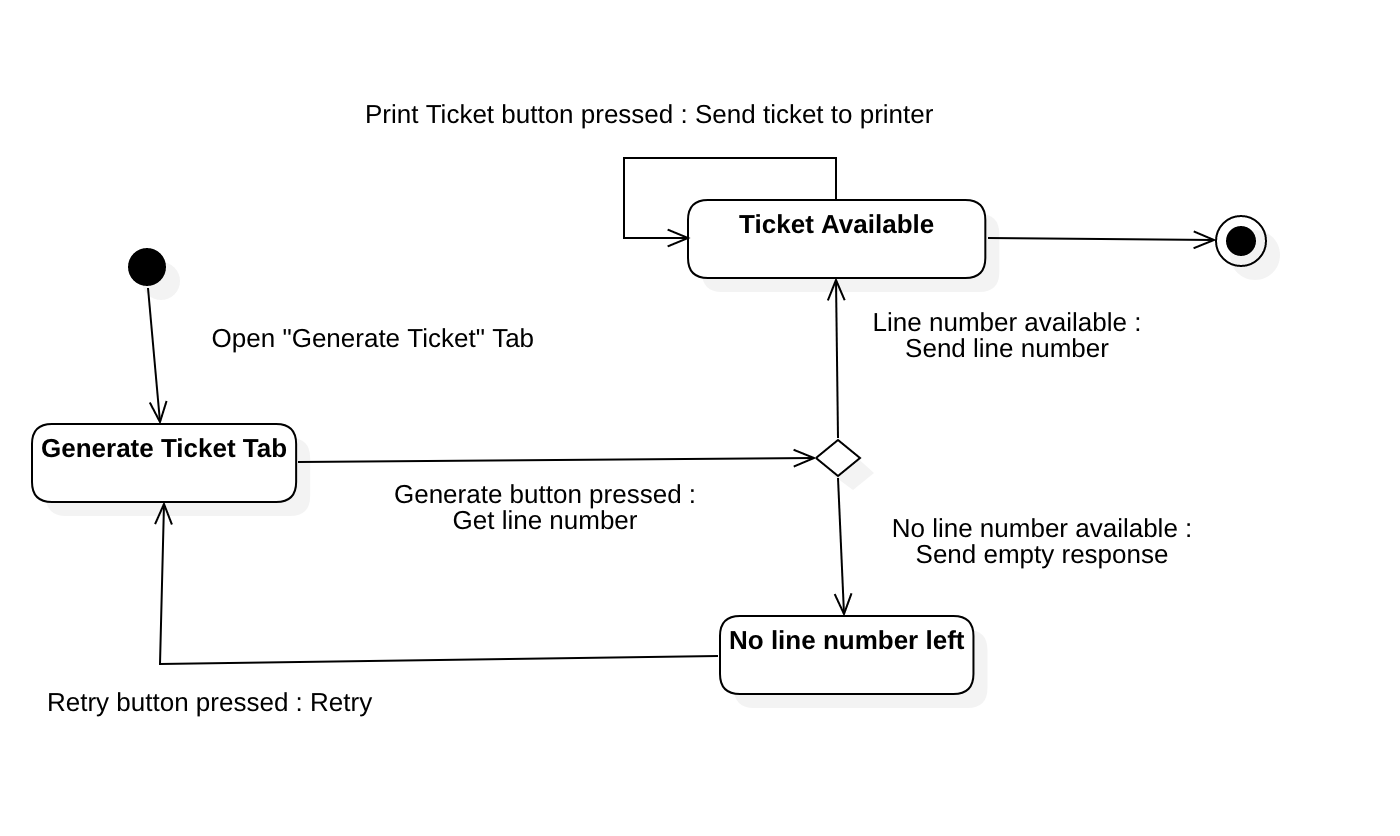
\includegraphics[height=0.4\textwidth]{Images/StateCharts/PrintTicket.png}
    \caption{State Diagram for feature Print Line Number}
    \label{fig:SDPrintLine}
\end{figure}

The \nameref{fig:SDPrintLine} represents the execution flow of a similar use case, printing an actual ticket for on foot visitors.
Upon arrival of a new customer that doesn't have a line number, the clerk opens the generate ticket tab and presses the "Generate" button to create a new line number.
Then, if all the constraints are satisfied the system allocates a new ticket number for the customer.
The clerk can then print the ticket out using a printer.
In case there are no line numbers left, the system notifies the clerk as such, with an option to retry the operation.

\subsubsection{System Stop}

\textbf{Scenario}

Gianfranco is a team lead in a shoe factory.
The shoe factory also has an outlet store, where the local brand sells its shoes directly to customers in a discounted price.
One day, a fire erupts due to a malfunction in the automated sewing machine and it starts to spread all over the building.
Gianfranco coordinates the evacuation of the factory and the store.
He also uses the CLup app to issue a system stop to prevent further customers from flooding in.
All the customers of the store receive notification regarding this unfortunate event, and don't arrive at the location.

\textbf{State Chart}

\begin{figure}[H]
    \centering
    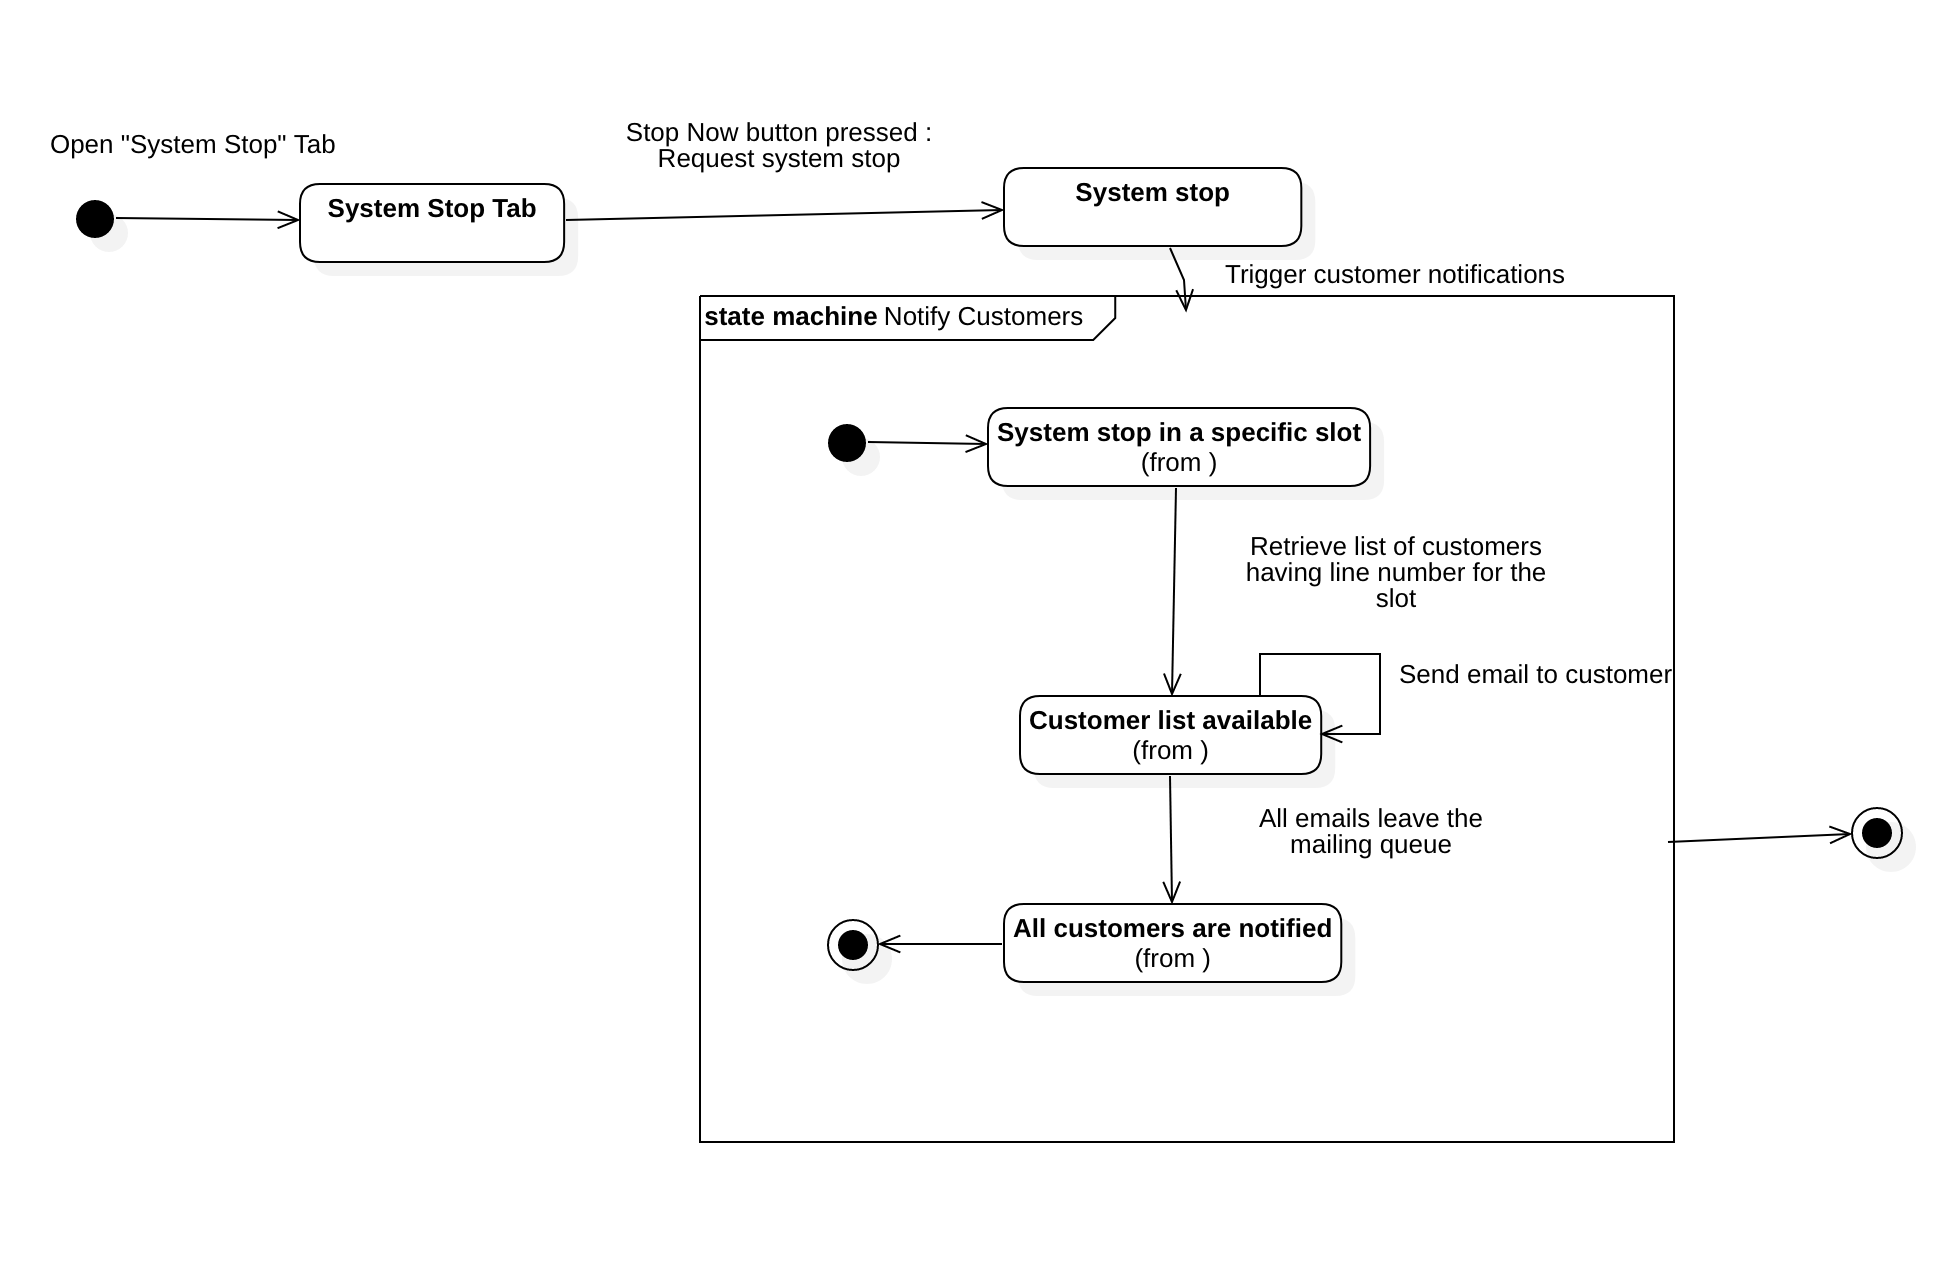
\includegraphics[height=0.4\textwidth]{Images/StateCharts/SystemStop.png}
    \caption{State Diagram for feature System Stop}
    \label{fig:SDSystemStop}
\end{figure}

The \nameref{fig:SDSystemStop} represents the execution flow for an important use case, the ability of the manager to halt the system, so that all line numbers gets cancelled, all users notified and no further line numbers are issued.
The manager first opens the System Stop tab on their phone, and afterwards request a system stop.
This action stops the system from issuing more tickets and triggers distribution of notifications for the time zones the system is stopped in.
In the notification part of the state diagram, the system starts with a request for stop for a specific time slot, and using that retrieves all the customers that have already scheduled for that slot.
The system, then starts sending emails to all customers that are in the list provided.
When all emails leave the mailing queue, the system has successfully notified all the customers regarding the stop.
The state machine of Notifying Customers is re-used to describe the notification mechanism in the \nameref{fig:SDScheduleStop}.

\subsubsection{Schedule System Stop}

\textbf{Scenario}

Giuseppe is an owner of a famous local pizza place.
He is using the CLup system in his store to manage the customer lines.
He is also preparing a new radio advertisement for his store, with an advertisement agency.
They have a meeting next week during work hours and he doesn't have anyone to give the authority to manage the store.
Therefore, he has to shut the store down for half the day.
He schedules a system stop from the CLup system to prevent any ticket numbers being issued in that day for his store.

\textbf{State Chart}

\begin{figure}[H]
    \centering
    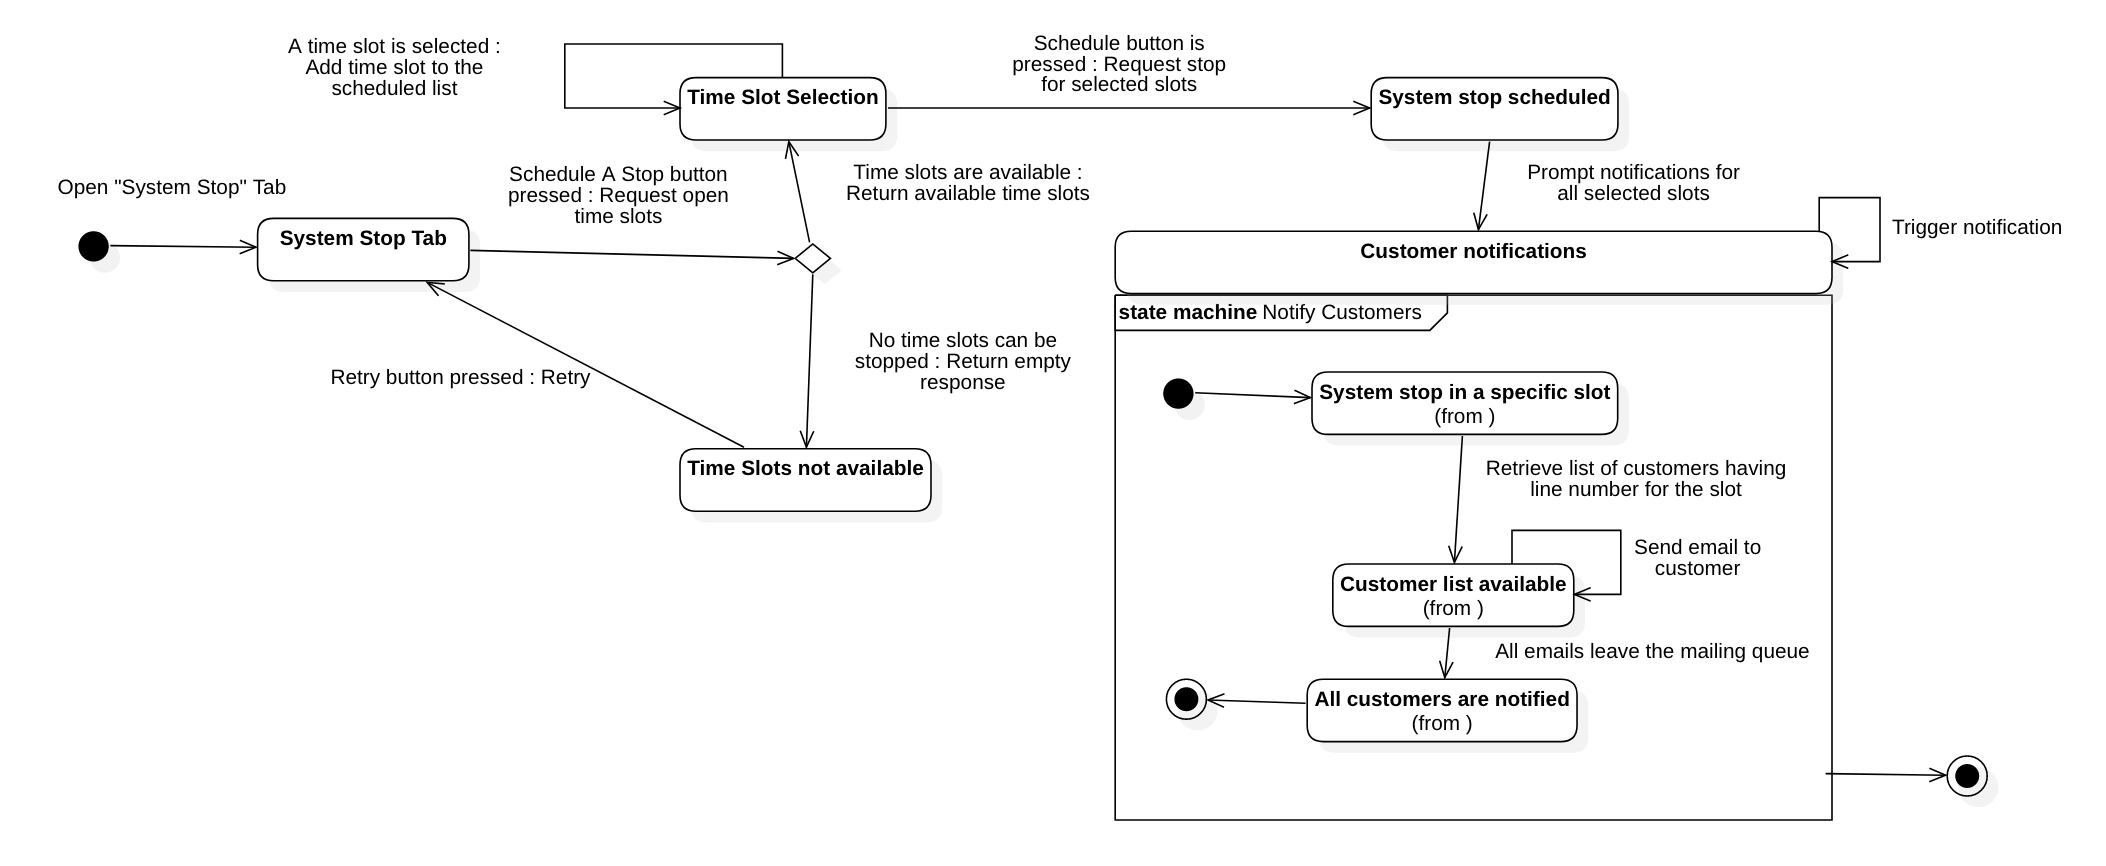
\includegraphics[height=0.4\textwidth]{Images/StateCharts/ScheduleSystemStop.png}
    \caption{State Diagram for feature Schedule System Stop}
    \label{fig:SDScheduleStop}
\end{figure}

The \nameref{fig:SDScheduleStop} represents the final core use case of the system that is considered as significant, scheduling the system to stop in the future.
To start this flow, the manager first opens the System Stop tab and presses the schedule a stop button.
The system than pools all the available slots that the manager can issue a stop on, and returns the list to the time slot selection screen.
If no such slot is available, a screen indicating such a case is visible, with an opportunity to retry the action.
From the time slot selection list, the manager selects specific time slots that the system shall stop for, and press Schedule button to schedule the system stop.
A scheduled system stop also sends a notification to all customers that have booked a time slot for that shop before the system stop.
The mechanism of customer notification is detailed in the description of the \nameref{fig:SDSystemStop}, so it will not be repeated here.
% here  we  include scenarios  and further details on the shared phenomena and a domain model (class diagrams and state charts)


\subsection{Product functions}
% TODO: @Hrvoje do these 3

% subsubsections with functions of (some?) requirements
% here we include the most important requirements
% for requirements use the R_1, R_2, R_3 syntax


\subsection{User characteristics}
% User roles: Manager & User & Clerk (& maybe unregistered user?)

% People need to be able to use Tickets, maybe: %90 / %10
% here we include anything that is relevant to clarify their needs


\subsection{Assumptions,dependencies and constraints}
\subsubsection{Domain Assumptions}

\begin{itemize}
    \item \textbf{$D_1$} \%80 of the customers and all clerks and managers have basic ICT skills, has an email address that they are willing to use to authenticate to the system and has a smart phone or equivalent device that can connect to the Internet, have a browser that supports UTF-8, display QR codes and has a mapping application. % All cases
    \item \textbf{$D_2$} Locations will not be visited by no more than 1000 people in any time slot. % Line number limit, we can provide 000-999 as numbers
    \item \textbf{$D_3$} \%98 of the customers will arrive at the given location either without a ticket or with a ticket that has not timed out. % Timeout policy
    \item \textbf{$D_4$} E-mail addresses are not shared by multiple users of the system. % Registeration, user info
    \item \textbf{$D_5$} Clerks' mobile devices are equipped with at least one camera that the system can use. % For QR code detection
    \item \textbf{$D_6$} All users have a basic understanding of how the line numbering system works and respects the ordering provided by the system. % The core use case
    \item \textbf{$D_7$} Managers have an estimate for the amount of reservations that their location can at most have. % To set a maximum amount of clients
    \item \textbf{$D_8$} Managers' device has location services that has a location acquisition error for no more than 20 meters. % To set the location accurately
    \item \textbf{$D_9$} Clerks are constantly monitoring the locations entrances and exits. % For QR code reading to take customers in and out
    \item \textbf{$D_{10}$} Locations have printing equipments that are in 5 meters range of all the entrances that can print QR codes and line numbers. % To print tickets
    \item \textbf{$D_{12}$} At least one manager is available in the location during the working hours. % To monitor and shutdown during emergencies
    \item \textbf{$D_{13}$} The customer's entry and exit to the store is determined by whether the clerks have checked them in and out.
    \item \textbf{$D_{14}$} The customer has their line number or line number ticket available with them through their visit, including their exit from the store % (no dead battery, printed ticket loss, etc)
\end{itemize}
% here we include domain assumptions
% use the D_1, D_2,... syntax
\subsubsection{Dependencies}
% TODO: @Hrvoje these 2 too.
% Maps API
% What external libraries, tools, integrations does the system rely on
\subsubsection{Constraints}
% Maps API failure
% All user and location info can be represented with UTF-8 character encoding.
% What are the limits imposed by the environment, regulatory policies, hardware & software limitations, etc...
